\documentclass[12pt]{article}

\usepackage[a4paper,margin=2.5cm]{geometry}
\usepackage{amsmath, amssymb, amsthm}
\usepackage{bm}
\usepackage{hyperref}
\usepackage{graphicx}
\usepackage{caption}
\usepackage{listings}
\usepackage{xcolor}
\usepackage{float}
\usepackage{placeins}
\graphicspath{{figures/}}

\lstdefinestyle{code}{
  basicstyle=\ttfamily\small,
  numbers=left,
  numberstyle=\tiny,
  numbersep=8pt,
  keywordstyle=\color{blue},
  commentstyle=\color{teal!70!black},
  stringstyle=\color{orange!70!black},
  showstringspaces=false,
  breaklines=true,
  frame=single,
  framerule=0.3pt,
  rulecolor=\color{black!15}
}
\lstset{style=code}

\title{Deep Q-Network (DQN) Tutorial}
\author{}
\date{\today}

\begin{document}
\maketitle

\section{Introduction}
Deep Q-Networks (DQNs) approximate the optimal action-value function using deep neural networks combined with experience replay and target networks. DQNs enable reinforcement learning in high-dimensional observation spaces such as images by stabilizing temporal-difference learning with these techniques.

\section{Theory and Formulas}
\subsection{Value Approximation}
Given network \(Q_\theta(s,a)\) and target network \(Q_{\theta^-}(s,a)\), the squared temporal-difference loss for transition \((s,a,r,s')\) is
\begin{equation}
L(\theta) = \Big( r + \gamma \max_{a'} Q_{\theta^-}(s',a') - Q_\theta(s,a) \Big)^2.
\end{equation}
Gradients are accumulated over mini-batches sampled from a replay buffer \(\mathcal{D}\).

\subsection{Target Network Updates}
Target parameters are updated either periodically or via Polyak averaging:
\begin{equation}
\theta^- \leftarrow \tau \theta + (1-\tau) \theta^-.
\end{equation}
Using a slowly moving target mitigates divergence due to correlated updates.

\subsection{Experience Replay}
Transitions collected during interaction are stored in a replay buffer. Sampling uniform mini-batches breaks correlation, improves sample efficiency, and accelerates convergence. Extensions such as prioritized replay weigh samples by TD-error magnitude.

\section{Applications and Tips}
\begin{itemize}
  \item \textbf{Atari game playing}: original DQN achieved human-level performance using raw pixels.
  \item \textbf{Robotics and simulation}: discretized action spaces for control tasks.
  \item \textbf{Operations research}: decision problems with structured observations.
  \item \textbf{Best practices}: normalize inputs, clip rewards, anneal exploration rate, monitor loss and TD-errors, and employ gradient clipping.
\end{itemize}

\section{Python Practice}
The script \texttt{gen\_dqn\_figures.py} trains a small neural-network DQN on a one-dimensional control task with discretized actions. It logs episode returns and visualizes the learned state-action value estimates.
\begin{lstlisting}[language=Python,caption={Excerpt from gen_dqn_figures.py}]
q_target = reward + gamma * np.max(target_network(next_state), axis=0)
q_values = online_network(state)
loss = mse(q_target, q_values[action])
optimizer.zero_grad(); loss.backward(); optimizer.step()
\end{lstlisting}

\section{Result}
\begin{figure}[H]
  \centering
  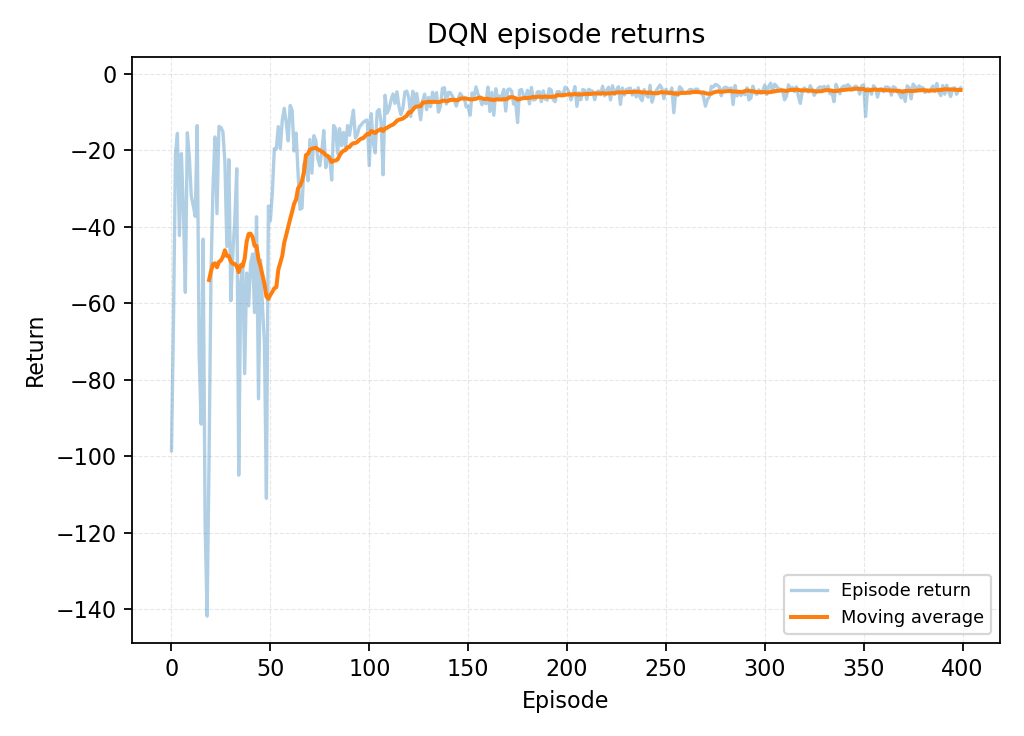
\includegraphics[width=0.8\linewidth]{dqn_returns.png}
  \caption{DQN episode returns converging toward optimal control}
  \label{fig:dqn_returns}
\end{figure}

\begin{figure}[H]
  \centering
  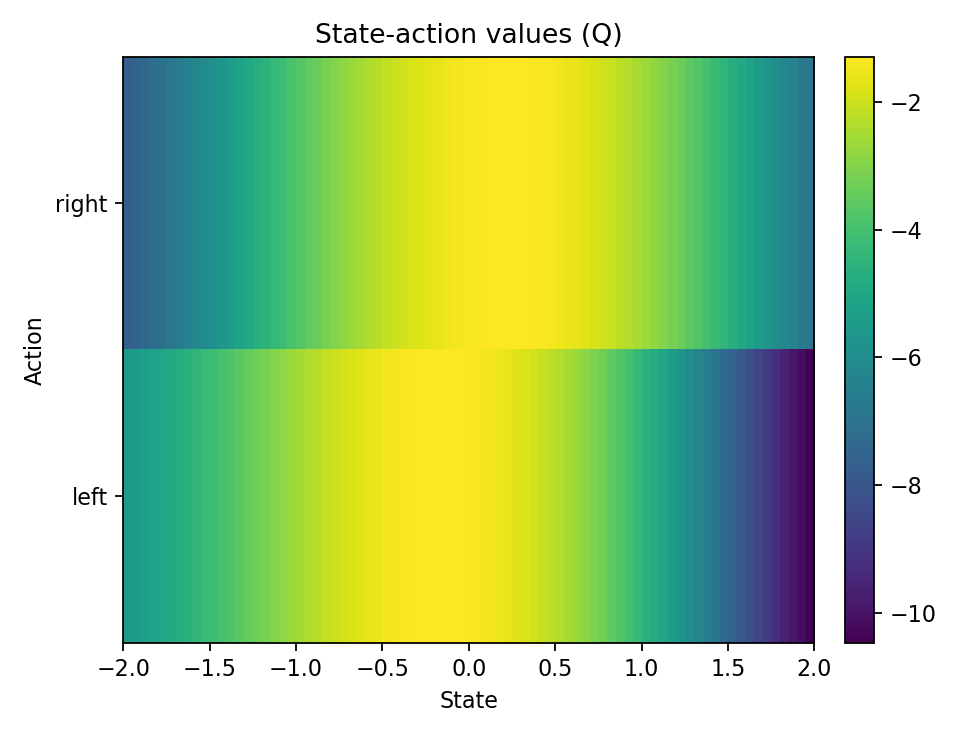
\includegraphics[width=0.82\linewidth]{dqn_q_values.png}
  \caption{State-action value heatmap learned by the DQN}
  \label{fig:dqn_q_values}
\end{figure}

\FloatBarrier
\section{Summary}
DQN stabilizes deep value learning via replay buffers and target networks, enabling high-dimensional control tasks. Proper tuning of learning rate, exploration, and update schedules ensures convergence. The toy control example demonstrates increasing returns and interpretable Q-values across the state space.

\end{document}